\section{Geometric Preliminaries}
\label{sec:rgpc}
In this section, we review some basic concepts in differential geometry that serve as cornerstones for our method. We refer to standard differential geometry textbooks for more details~\cite{do1992riemannian,fecko2006differential}.

\subsection{Riemannian Manifolds}

\begin{figure}[!t]
    \centering
    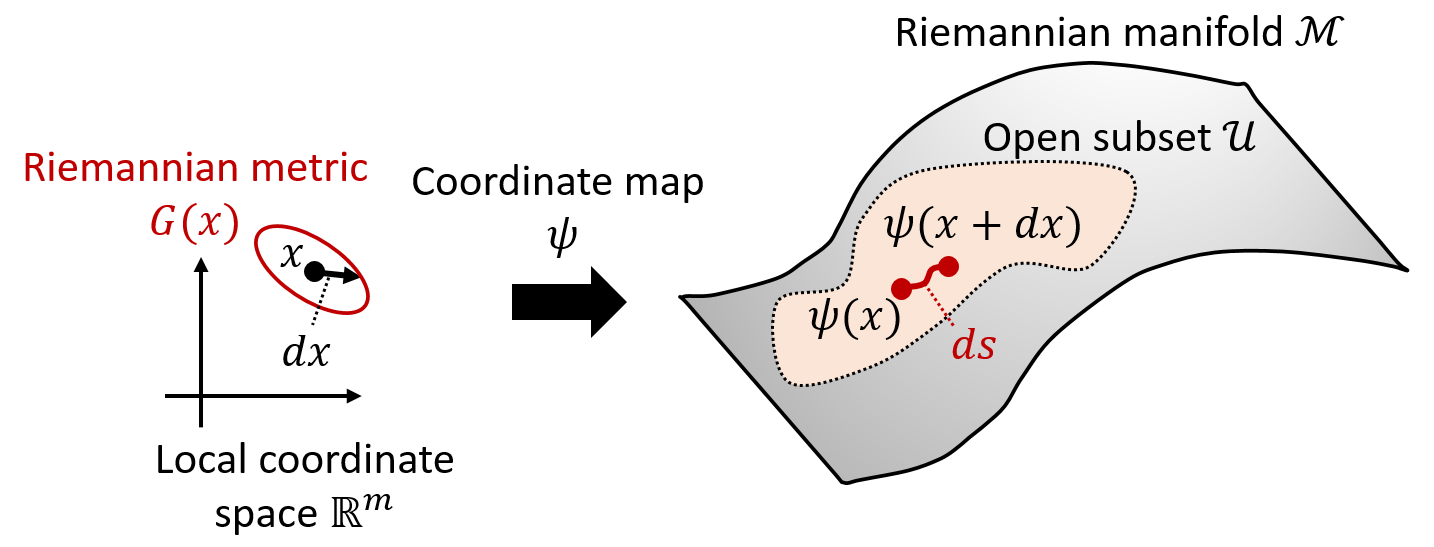
\includegraphics[width=\linewidth]{figure/gp1.PNG}
    \caption{A local coordinate system for an $m$-dimensional Riemannian manifold ${\cal M}$. The Riemannian metric at coordinates $x$, $G(x)$, is visualized as a red equidistant ellipse that is $\{y \in \mathbb{R}^{m} \: | \: (y-x)^T G(x) (y-x) = {\rm constant}\}$.}
    \label{fig:gp1}
\end{figure}
A smooth manifold ${\cal M}$ equipped with a positive-definite inner product on the tangent space at each point is called a {\it Riemannian manifold}, and the family of inner products is called a {\it Riemannian metric}.
Given an $m$-dimensional Riemannian manifold ${\cal M}$ and its local coordinates $x \in \mathbb{R}^{m}$ -- when using local coordinates, we implicitly assume there exists a local coordinate map $\psi:\mathbb{R}^{m} \to {\cal U} \subset {\cal M}$ --, the Riemannian metric at $x$ can be expressed as an $m\times m$ positive-definite matrix denoted by $G(x) \in \mathbb{R}^{m \times m}$; see Fig.~\ref{fig:gp1}. This defines several geometric notions on ${\cal M}$, such as lengths, angles, and volumes. For example, given an infinitesimal displacement vector $dx \in \mathbb{R}^{m}$, its squared length is defined as follows:
\begin{equation}
    ds^2 = dx^T G(x) dx = \sum_{i,j=1}^{m} g_{ij}(x)dx^i dx^j,
\end{equation}
where $\{g_{ij}(x)\}$ is an index notation of the matrix $G(x)$ and $dx = (dx^1, \ldots, dx^m)$.

\subsection{Immersion and Embedding}
\label{sec:iande}
\begin{figure}[!t]
    \centering
    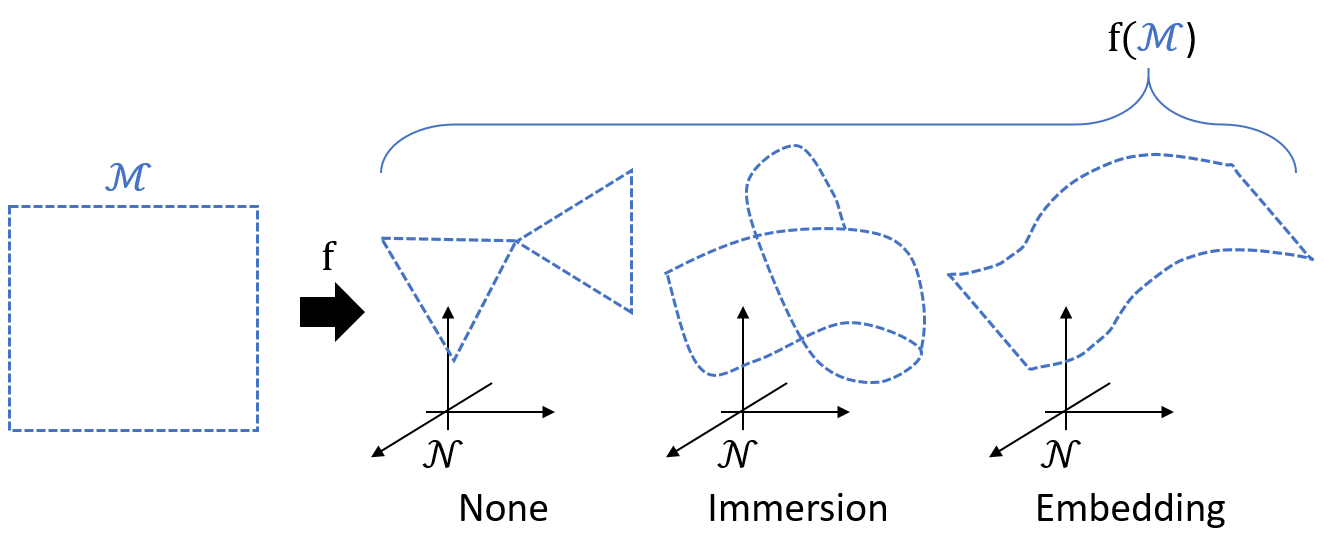
\includegraphics[width=\linewidth]{figure/gp2.PNG}
    \caption{An illustration of immersion and embedding between two manifolds ${\cal M}$ and ${\cal N}$.}
    \label{fig:gp2}
    \vspace{-5pt}
\end{figure}
Consider two differentiable manifolds, an $m$-dimensional manifold ${\cal M}$ and $n$-dimensional manifold ${\cal N}$, with their respective coordinates $x\in\mathbb{R}^{m}$ and $y \in \mathbb{R}^{n}$. A differentiable mapping ${\rm f}:{\cal M} \to {\cal N}$ is an {\it immersion} if its differential is an injective function at every point in ${\cal M}$. Representing the mapping in local coordinates as $f:\mathbb{R}^{m} \to \mathbb{R}^{n}$, equivalently, $f$ is an immersion if its Jacobian matrix
\begin{equation}
    J(x):=\frac{\partial f}{\partial x}(x) \in \mathbb{R}^{n \times m}
\end{equation}
has constant rank equal to $\text{dim}({\cal M})=m$ at every point. Intuitively, for $f$ to be an immersion, the output manifold dimension $n$ must be greater or equal to the dimension of ${\cal M}$. 
A smooth {\it embedding} is an injective immersion ${\rm f}:{\cal M} \to {\cal N}$ such that ${\cal M}$ is diffeomorphic to its image ${\rm f}({\cal M}) \subset {\cal N}$\footnote{A manifold ${\cal A}$ is diffeomorphic to another manifold ${\cal B}$ if there exists a differentiable map between ${\cal A}$ and ${\cal B}$ such that its inverse exists and is differentiable as well.}. Specifically, when the domain manifold is compact, a smooth embedding is equivalent to an injective immersion. Then, ${\rm f}({\cal M})$ is called an {\it embedded manifold} in ${\cal N}$; see Fig.~\ref{fig:gp2}. 

% When ${\cal N}$ is a Riemannian manifold with a Riemannian metric $H(y)=\{h_{ij}(y)\}$ expressed in local coordinates $y \in \mathbb{R}^{n}$, and if there exists an embedding ${\rm f}:{\cal M} \to {\cal N}$, an embedded manifold ${\rm f}({\cal M})$ can naturally inherit the Riemannian geometry form ${\cal N}$. 
% Let $x \in \mathbb{R}^{m}$ be local coordinates for ${\cal M}$ with a coordinate map $\psi:\mathbb{R}^{m} \to {\cal U} \subset {\cal M}$. Then, with a new coordinate map ${\rm f} \circ \psi : \mathbb{R}^{m} \to {\rm f}({\cal U}) \subset {\rm f}({\cal M})$, we can treat $x$ as local coordinates for the embedded manifold as well.
% If we denote by $G(x)$ the Riemannian metric in $ {\rm f}({\cal M})$ inherited from ${\cal N}$ in local coordinates, the following equality holds:
% \begin{equation}
%     ds^2 = dx^T G(x) dx = dy^T H(y) dy
% \end{equation}
% for all $x$ and $dx$, where $y=f(x)$ and $dy=J(x)dx$. Therefore, $G(x)=J^T(x)H(f(x))J(x)$ which is called a {\it pullback metric}.

\subsection{Riemannian Geometry of Parametric Curves}
\label{sec:rgpc}

\begin{figure}[!t]
    \centering
    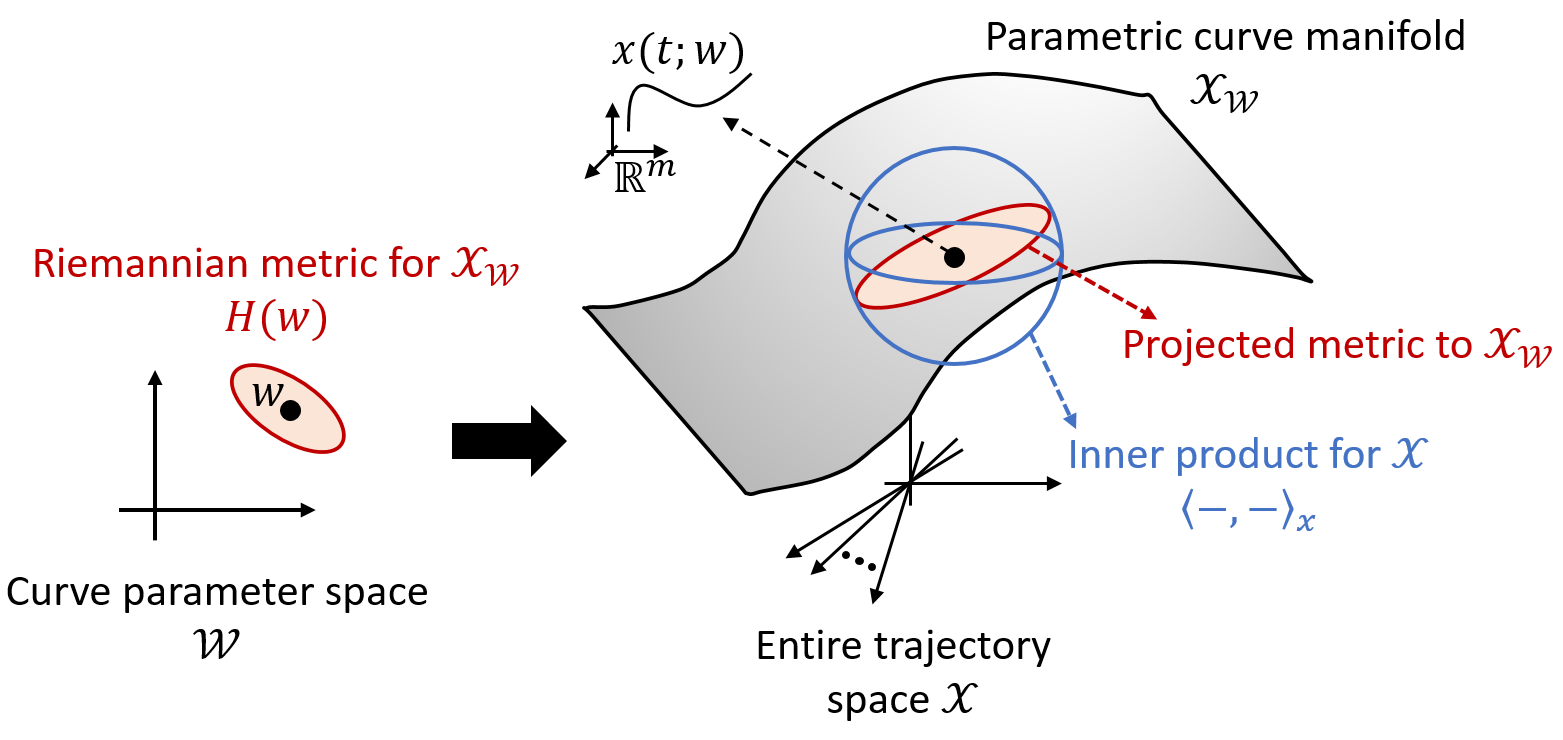
\includegraphics[width=\linewidth]{figure/gp3.PNG}
    \caption{An illustration of Riemannian geometry of the parametric curve manifold ${\cal X}_{\cal W}$.}
    \label{fig:gp3}
    \vspace{-5pt}
\end{figure}

In this paper, we are particularly interested in Riemannian geometry of manifold of parametric curves. This section introduces how to define a Riemannian metric for the parametric curve manifold; see Fig.~\ref{fig:gp3}.

Let ${\cal M}$ be an $m$-dimensional Riemannian manifold with its local coordinates $x \in \mathbb{R}^{m}$ and Riemannian metric $G(x)$. Consider a smooth curve in ${\cal M}$ expressed as $x:[0, T] \to \mathbb{R}^{m}$ in coordinates, where its velocity norm is defined as $\|\dot{x}\|:=\sqrt{\dot{x}^T G(x) \dot{x}}$. 
The space of all smooth curves is considered an infinite-dimensional function space ${\cal X}$ with an inner product defined as follows: $\langle v, w \rangle_x:= \int_{0}^{T} v(t)^T G(x(t)) w(t) \ dt$ for two square-integrable functions $v,w:[0,T] \to \mathbb{R}^{m}$ (i.e., ${\cal X}$ is a Hilbert space). 

Of particular relavance to this paper is a parametric curve $x(t; w)$ where $w \in {\cal W}$ denotes the parameter of the curve and ${\cal W} \subset \mathbb{R}^{n}$. Consider the set of all parametric curves ${\cal X}_{{\cal W}} := \{x(\cdot;w) \in {\cal X} \ | \ w \in {\cal W}\}$. This space is a $n$-dimensional smooth manifold under the following conditions:
\begin{prop}
\label{prop:manifold}
    Suppose a curve $x(t;w)$ is smooth in both $t$ and $w$ and $x(t;\cdot): {\cal W} \to {\cal X}$ is injective, i.e., if $x(t;w_1)=x(t;w_2)$ for all $t \in [0, T]$, then $w_1 = w_2$. Let $w=(w^1,\ldots, w^n)$ and $v=(v^1,\ldots, v^n)\in \mathbb{R}^{n}$, if 
    \begin{equation}
    \label{eq:immersion}
        \sum_{i=1}^{D} \frac{\partial x(t;w)}{\partial w^{i}} v^{i} = 0 \:\:\: \implies \:\:\: v=0
    \end{equation}
    for all $w \in {\cal W}$ and ${\cal W}$ is compact, then ${\cal X}_{{\cal W}}$ is an $n$-dimensional smooth manifold. 
\end{prop}

\begin{proof}
    A smooth map $x(t; \cdot): {\cal W} \to {\cal X}$ is an injective immersion by (\ref{eq:immersion}). Since ${\cal W}$ is compact, the mapping is an embedding (i.e., ${\cal X}_{{\cal W}}$ is an embedded manifold in ${\cal X}$). 
\end{proof}

Given a parametric curve manifold ${\cal X}_{\cal W}$ embedded in ${\cal X}$, the inner product $\langle \cdot, \cdot \rangle_x$ in ${\cal X}$ can be naturally projected into ${\cal X}_{{\cal W}}$. This leads to -- by treating ${\cal W}$ as a local coordinate space for ${\cal X}_{{\cal W}}$ -- the Riemannian metric in ${\cal X}_{{\cal W}}$ expressed in the parameter space ${\cal W}$, denoted by $H(w)=\{h_{ij}(w)\}$. Specifically, the squared length of an infinitesimal displacement $dw \in \mathbb{R}^{n}$ is
\begin{align}
    ds^2 
    &= \sum_{i,j} h_{ij}(w) dw^i dw^j \nonumber \\ 
    &= \int_{0}^T \langle \sum_{i} \frac{\partial x(t;w)}{\partial w^i} dw^i,  \sum_{j} \frac{\partial x(t;w)}{\partial w^j} dw^j \rangle_x \ dt\nonumber \\
    &=\sum_{i,j} \Big( \int_{0}^T \frac{\partial x(t; w)^T}{\partial w^i} G(x(t;w))\frac{\partial x(t; w)}{\partial w^j} \ dt \Big) dw^i dw^j.
\end{align}
Therefore, 
\begin{equation}
\label{eq:rm}
    H(w) = \int_{0}^T \big( \frac{\partial x(t; w)}{\partial w}\big)^T G(x(t;w))\frac{\partial x(t; w)}{\partial w} \ dt,
\end{equation}
where $\frac{\partial x(t; w)}{\partial w} \in \mathbb{R}^{m\times n}$. 
This method of metric construction follows the standard procedure in differential geometry. A similar procedure can be found in the construction of Fisher information Riemannian metrics in statistical manifolds~\cite{amari2016information,lee2022statistical}.

\subsection{Isometry and Coordinate-Invariant Distortion Measure}
\begin{figure}[!t]
    \centering
    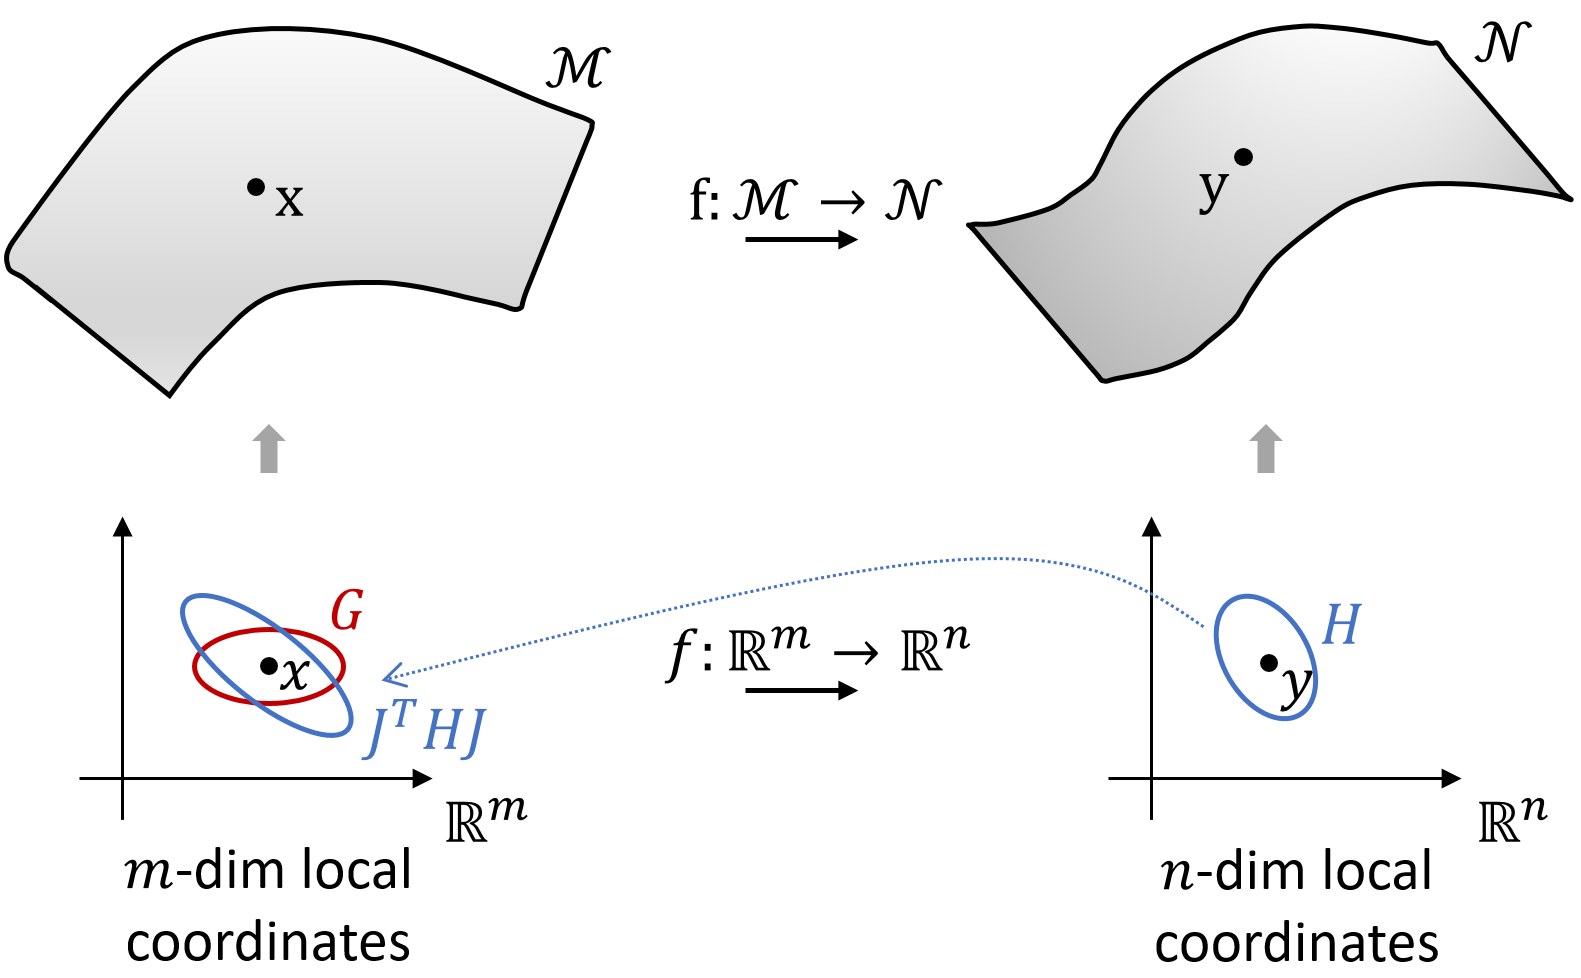
\includegraphics[width=0.85\linewidth]{figure/gp4.PNG}
    \caption{An illustration of a mapping between two Riemannian manifolds. If $G=J^THJ$, i.e., the red and blue ellipses coincide, at all points in $\mathbb{R}^{m}$, then the mapping $f$ is a global  isometry.}
    \label{fig:gp4}
    \vspace{-5pt}
\end{figure}

Consider two Riemannian manifolds, an $m$-dimensional manifold ${\cal M}$ with local coordinates $x\in\mathbb{R}^{m}$ and metric $G(x)$ and an $n$-dimensional manifold ${\cal N}$ with local coordinates $y\in\mathbb{R}^{n}$ and metric $H(y)$. And let $f:\mathbb{R}^{m} \to \mathbb{R}^{n}$ be a differentiable mapping between two manifolds expressed in local coordinates. 

We call $f$ an {\it isometry} if it preserves geometric structures between two spaces, i.e., preserves distances, angles, and volumes. Specifically, let $J(x)=\frac{\partial f}{\partial x}(x)$, if 
\begin{equation}
    G(x) = J(x)^T H(f(x)) J(x)
\end{equation}
at $x$, then $f$ is called a local isometry at $x$ (to see why, compare $dx^TG(x)dx$ and $dy^T H(y)dy$ where $dy=J(x)dx$). If this condition is satisfied at all points in ${\cal M}$, then $f$ is a (global) isometry; see Fig.~\ref{fig:gp4}. 

Sometimes, it is too stringent to find an isometry between two spaces and better to ignore the scale of distances~\cite{yonghyeon2022regularized}. A mapping $f$ that satisfies the relaxed condition
\begin{equation}
\label{eq:lsic}
    G(x) = cJ(x)^T H(f(x)) J(x)
\end{equation}
for all $x$ and for some positive scalar $c$ is called a {\it scaled isometry}. It preserves, angles and scaled distances.

There is a family of coordinate-invariant Riemannian {\it distortion measures}, each of which is a functional of a mapping $f$ that measures how far $f$ from being an isometry~\cite{jang2021riemannian}. 
Let $\lambda_i$ be eigenvalues of $J^T H J G^{-1}$. One example is  
\begin{equation}
    \int_{\cal M} \|\lambda_i(x) - 1\|^2 \sqrt{\det G(x)} dx.
\end{equation}
This measure is coordinate-invariant\footnote{To see why, consider a pair of coordinate transformations $\psi: x\mapsto x'$ and $\phi: y \mapsto y'$. Let $\Psi = \frac{\partial \psi}{\partial x}$ and $\Phi=\frac{\partial \phi}{\partial y}$, then the Riemannian metrics transform via $G\mapsto \Psi^{-T} G \Psi^{-1}$ and $H\mapsto \Phi^{-T}H\Phi^{-1}$, while the Jacobian transforms via $J\mapsto \Phi J \Psi^{-1}$. Therefore, $J^T H J G^{-1} \mapsto \Psi^{-T}J^T H J G^{-1}\Psi^{T}$ and the eigenvalues remain unchanged.}, and note that if $\lambda_i(x)=1$ for all $x$, then the measure is zero and $f$ is an isometry.

A family of {\it relaxed distortion measures} quantifies how far $f$ from being a scaled isometry~\cite{yonghyeon2022regularized} within the support of a positive finite measure $\nu$ in ${\cal M}$. One of them is
\begin{equation}
\label{eq:rdm}
    \int_{\cal M} \|\frac{\lambda_i(x)}{\frac{1}{\nu({\cal M})}\int_{\cal M} \frac{1}{m}\sum_{i=1}^{m} \lambda_i(x) d\nu(x)} - 1\|^2 d\nu(x).
\end{equation}
This measure is coordinate-invariant, and note that if $\lambda_i(x)=c$ for all $x$ in the support of $\nu$ for some positive scalar $c$, then the measure is zero and $f$ is a scaled isometry in $\nu$ (i.e., equation (\ref{eq:lsic}) is satisfied at all points in the support of $\nu$). 

Given a probability measure $P$ in ${\cal M}$, restricting the relaxed distortion measure~(\ref{eq:rdm}) to the support of $P$ and removing the additive constant, it is proportional to 
\begin{equation}
\label{eq:rdmff}
    {\cal R}(f; P):=\frac{\mathbb{E}_{x \sim P} [{\rm Tr} \big((J^THJG^{-1})^2\big)]}{\mathbb{E}_{x\sim P}[{\rm Tr}\big(J^THJG^{-1}\big)]^2}.
\end{equation}
Given this trace-based expression, we can employ the Hutchinson stochastic trace estimator, i.e., $\text{Tr}(A) = \mathbb{E}_{v\sim {\cal N}(0, I)}[v^T A v]$, which facilitates an efficient implementation of isometric regularization. Further details can be found in~\cite{lee2023equivariant,lee2023geometric}.